\subsection*{Kinetic Models}
    \line
    \begin{definition}[Kinetic model]
        Here, ``kinetic'' models refer to those wherein the distribution of particles positions and velocities is modelled through a single distribution function, as a function of both position and velocity.
    \end{definition}
    \line
    For each phase, $s$, we define the distribution functions $(f_{s}(\bfx, \bfv; t))_{s}$
    \begin{equation}
        f_{s}(\bfx, \bfv; t)  :=  \sum_{i}\delta^{3}(\bfx - \bfx_{si})\delta^{3}(\bfv - \bfv_{si})
    \end{equation}
    While working with such $(f_{s})_{s}$ could \emph{in theory} be used to model all the particles exactly and simultaneously, variations in $\bfx$ of each $f_{s}$ occur on the length scale of the distances between particles, i.e. on the order of $10^{- 6}\rmm$ in a tokamak plasma. We would therefore need a mesh resolution on a similar (if not finer) length scale to capture the physical nature of each $f_{s}$. Again: computationally infeasible.

    Since, however, the \emph{precise} position of each particle is generally irrelevant to the general fluid behavior when not working on the atomic scale (in particular on tokamak plasma scales) the key idea of kinetic theory is to model this distribution function as a \emph{random} distribution, as one might do in Bayesian statistics to model a parameter that is known to be of fixed value as a random variable when full information on it remains unknown. One defines the 1-particle distribution functions, denoted here as $\left(\widetilde{f_{s}}(\bfx, \bfv; t)\right)_{s}$, such that $\forall \phi(\bfx, \bfv; t)$,
    \begin{equation}
        \bbE\left\{\int_{\bfx, \bfv; t}f_{s}(\bfx, \bfv; t)\phi(\bfx, \bfv; t)\right\}
        \left(=  \sum_{i}\bbE\{\phi(\bfx_{si}, \bfv_{si}; t)\}\right)
        =  \int_{\bfx, \bfv; t}\widetilde{f_{s}}(\bfx, \bfv; t)\phi(\bfx, \bfv;t )
    \end{equation}
    Similarly the electromagnetic field must be modeled as a random distribution, with $\widetilde{\bfE}(\bfx, t)$, $\widetilde{\bfB}(\bfx, t)$ defined, such that $\forall \bfphi(\bfx, t)$,
    \begin{align}
        \bbE\left\{\int_{\bfx; t}\bfE(\bfx, t)\cdot\bfphi(\bfx, t)\right\}  =  \int_{\bfx; t}\widetilde{\bfE}(\bfx, t)\cdot\bfphi(\bfx, t)  \\ 
        \bbE\left\{\int_{\bfx; t}\bfB(\bfx, t)\cdot\bfphi(\bfx, t)\right\}  =  \int_{\bfx; t}\widetilde{\bfB}(\bfx, t)\cdot\bfphi(\bfx, t)
    \end{align}
    We seek to cast the exact equations in $(f_{s})_{s}$, $\bfE$, $\bfB$ into ones in the distribution parameters $\left(\widetilde{f_{s}}\right)_{s}$, $\widetilde{\bfE}$, $\widetilde{\bfB}$. To do so, once can apply the workflow as outline in Figure \ref{fig:kinetic model construction workflow} to each equation.
    \begin{figure}[!ht]
        \centering
        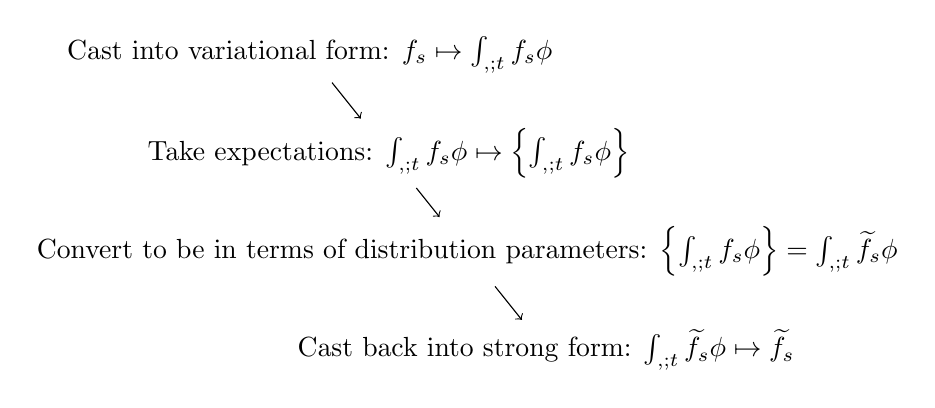
\begin{tikzpicture}[align = center, auto]
            \node (1) at (0, 0) {Cast into variational form: $f_{s}  \mapsto  \int_{\bfx, \bfv; t}f_{s}\phi$};
            \node (2) at (1, -1.25) {Take expectations: $\int_{\bfx, \bfv; t}f_{s}\phi  \mapsto  \bbE\left\{\int_{\bfx, \bfv; t}f_{s}\phi\right\}$};
            \node (3) at (2, -2.5) {Convert to be in terms of distribution parameters: $\bbE\left\{\int_{\bfx, \bfv; t}f_{s}\phi\right\}  =  \int_{\bfx, \bfv; t}\widetilde{f_{s}}\phi$};
            \node (4) at (3, -3.75) {Cast back into strong form: $\int_{\bfx, \bfv; t}\widetilde{f_{s}}\phi  \mapsto  \widetilde{f_{s}}$};

            \draw[->] (1) -- (2);
            \draw[->] (2) -- (3);
            \draw[->] (3) -- (4);
        \end{tikzpicture}
        \caption{Diagram of workflow for construction of a kinetic model}
        \label{fig:kinetic model construction workflow}
    \end{figure}

    Since this is entirely linear, Maxwell's equations—themselves linear—carry over identically:
    \begin{align*}
        \partial_{t}\widetilde{\bfE}  &=  c^{2}\nabla\wedge\widetilde{\bfB} - \frac{1}{\varepsilon_{0}}\sum_{s}q_{s}\int_{\bfv}\widetilde{f_{s}}\bfv,  &
        \partial_{t}\widetilde{\bfB}  &=  - \nabla\wedge\widetilde{\bfE}  \\
        \nabla\cdot\widetilde{\bfE}  &=  \frac{1}{\varepsilon_{0}}\sum_{s}q_{s}\int_{\bfv}\widetilde{f_{s}},  &
        \nabla\cdot\widetilde{\bfB}  &=  0
    \end{align*}
    The evolution equation for $\left(f_{s}{\color{white} \widetilde{f_{s}}}\!\!\!\!\!\right)_{s}$ or $\left(\widetilde{f_{s}}\right)_{s}$ is not so simple however, due to its non-linearity. When applying this technique we derive the ``\emph{Boltzmann equation}'', \BA{[Ref]}
    \begin{equation}\label{eqn:Boltzmann equation}
        \partial_{t}\widetilde{f_{s}} + \nabla_{\bfx}\cdot\left[\widetilde{f_{s}}\bfv\right] + \frac{q_{s}}{m_{s}}\nabla_{\bfv}\cdot\left[\widetilde{f_{s}}\left(\widetilde{\bfE} + \bfv\wedge\widetilde{\bfB}\right)\right]  =   \frac{q_{s}}{m_{s}}\sum_{s'}q_{s'}(\nabla_{\bfv}\cdot\bfC_{ss'})
    \end{equation}
    where the collision terms $(\bfC_{s}(\bfx, \bfv; t))_{s}$ are terms characterising the Coulomb collisions, defined as
    \begin{multline}\label{eqn:collision operator}
        \bfC_{ss'}  :=  \int_{\bfx' \neq \bfx, \bfv'; t'}\left(\widetilde{f_{s}}(\bfx, \bfv; t)\widetilde{f_{s'}}(\bfx', \bfv'; t') - \widetilde{f_{s}f_{s'}}[(\bfx, \bfv; t), (\bfx', \bfv'; t')]\right)  \\
        [\bfk_{\bfE}(\bfx' - \bfx, \bfv'; t' - t) + \bfv\wedge\bfk_{\bfB}(\bfx' - \bfx, \bfv'; t' - t)]
    \end{multline}
    where in turn:
    \begin{itemize}
        \item  $\bfk_{\bfE}$, $\bfk_{\bfB}$, as functions in $\bfx'$, $\bfv'$, $t'$, are kernels of the electric and magnetic field, defined as the electric and magnetic fields produced at the origin by a unit point charge at position $\bfx'$ with velocity $\bfv'$ at time $t' \left(\in \left[-\frac{1}{c}\|\bfx'\|, 0\right]\right)$. \BA{(Explicit definition for $\bfk_{\bfE}$, $\bfk_{\bfB}$? Not really needed for the theory.)}
        
        \item  The 2-particle distributions functions $\left(\widetilde{f_{s_{1}}f_{s_{2}}}[(\bfx_{1}, \bfv_{1}; t_{1}), (\bfx_{2}, \bfv_{2}; t_{s})]\right)_{s_{1}s_{2}}$ are defined such that $\forall \phi[(\bfx_{1}, \bfv_{1}; t_{1}), (\bfx_{2}, \bfv_{2}; t_{2})]$,
        \begin{multline}
            \bbE\left\{\int_{\bfx_{1}, \bfv_{1}; t_{1}}\int_{\bfx_{2}, \bfv_{2}; t_{2}}f_{s_{1}}(\bfx_{1}, \bfv_{1}; t_{1})f_{s_{2}}(\bfx_{2}, \bfv_{2}; t_{2})\phi[(\bfx_{1}, \bfv_{1}; t_{1}), (\bfx_{2}, \bfv_{2}; t_{2})]\right\}  \\
            \left(=  \sum_{i_{1}, i_{2}}\bbE\{\phi[(\bfx_{s_{1}i_{1}}, \bfv_{s_{1}i_{1}}; t_{1}), (\bfx_{s_{2}i_{2}}, \bfv_{s_{2}i_{2}}; t_{2})]\}\right)  \\
            =  \int_{\bfx_{1}, \bfv_{1}}\int_{\bfx_{2}, \bfv_{2}}\widetilde{f_{s_{1}}f_{s_{2}}}[(\bfx_{1}, \bfv_{1}; t_{1}), (\bfx_{2}, \bfv_{2}; t_{2})]\phi[(\bfx_{1}, \bfv_{1}; t_{1}), (\bfx_{2}, \bfv_{2}; t_{2})]
        \end{multline}
        These capture the nature of how the positions of pairs of particles are correlated.
    \end{itemize}
    For a full derivation of (\ref{eqn:Boltzmann equation}) see Appendix \ref{cha:Boltzmann equation derivation}.

    Obviously this system is not closed, as it in turn is dependent on $\left(\widetilde{f_{s_{1}}f_{s_{2}}}\right)_{s_{1}s_{2}}$; this is referred to as the ``\emph{closure problem}''. Different approximations to $\left(\widetilde{f_{s_{1}}f_{s_{2}}}\right)_{s_{1}s_{2}}$ lead to different collisional forces and collision operators in the Boltzmann equation.

    From here, we shall drop the tildes $\widetilde{*}$ on $\widetilde{f_{s}}$, $\widetilde{\bfE}$, $\widetilde{\bfB}$.
    